\documentclass[11pt]{article}\usepackage[]{graphicx}\usepackage[]{color}
%% maxwidth is the original width if it is less than linewidth
%% otherwise use linewidth (to make sure the graphics do not exceed the margin)
\makeatletter
\def\maxwidth{ %
  \ifdim\Gin@nat@width>\linewidth
    \linewidth
  \else
    \Gin@nat@width
  \fi
}
\makeatother

\definecolor{fgcolor}{rgb}{0.345, 0.345, 0.345}
\newcommand{\hlnum}[1]{\textcolor[rgb]{0.686,0.059,0.569}{#1}}%
\newcommand{\hlstr}[1]{\textcolor[rgb]{0.192,0.494,0.8}{#1}}%
\newcommand{\hlcom}[1]{\textcolor[rgb]{0.678,0.584,0.686}{\textit{#1}}}%
\newcommand{\hlopt}[1]{\textcolor[rgb]{0,0,0}{#1}}%
\newcommand{\hlstd}[1]{\textcolor[rgb]{0.345,0.345,0.345}{#1}}%
\newcommand{\hlkwa}[1]{\textcolor[rgb]{0.161,0.373,0.58}{\textbf{#1}}}%
\newcommand{\hlkwb}[1]{\textcolor[rgb]{0.69,0.353,0.396}{#1}}%
\newcommand{\hlkwc}[1]{\textcolor[rgb]{0.333,0.667,0.333}{#1}}%
\newcommand{\hlkwd}[1]{\textcolor[rgb]{0.737,0.353,0.396}{\textbf{#1}}}%

\usepackage{framed}
\makeatletter
\newenvironment{kframe}{%
 \def\at@end@of@kframe{}%
 \ifinner\ifhmode%
  \def\at@end@of@kframe{\end{minipage}}%
  \begin{minipage}{\columnwidth}%
 \fi\fi%
 \def\FrameCommand##1{\hskip\@totalleftmargin \hskip-\fboxsep
 \colorbox{shadecolor}{##1}\hskip-\fboxsep
     % There is no \\@totalrightmargin, so:
     \hskip-\linewidth \hskip-\@totalleftmargin \hskip\columnwidth}%
 \MakeFramed {\advance\hsize-\width
   \@totalleftmargin\z@ \linewidth\hsize
   \@setminipage}}%
 {\par\unskip\endMakeFramed%
 \at@end@of@kframe}
\makeatother

\definecolor{shadecolor}{rgb}{.97, .97, .97}
\definecolor{messagecolor}{rgb}{0, 0, 0}
\definecolor{warningcolor}{rgb}{1, 0, 1}
\definecolor{errorcolor}{rgb}{1, 0, 0}
\newenvironment{knitrout}{}{} % an empty environment to be redefined in TeX

\usepackage{alltt}
\usepackage{amsmath}
\usepackage{pslatex}
\usepackage{natbib}
\usepackage{setspace}
%\usepackage[sc]{mathpazo}
%\usepackage[T1]{fontenc}
\usepackage[margin=1in,pdftex]{geometry}
\setcounter{secnumdepth}{2}
\setcounter{tocdepth}{2}
\usepackage{url}
\usepackage[unicode=true,pdfusetitle,
 bookmarks=true,bookmarksnumbered=true,bookmarksopen=true,bookmarksopenlevel=2,
 breaklinks=false,pdfborder={0 0 1},backref=false,colorlinks=false]{hyperref}
\hypersetup{pdfstartview={XYZ null null 1}}
\usepackage{breakurl}
\usepackage[utf8]{inputenc} 
%\usepackage[authoryear]{natbib}


\newcommand{\quanteda}{\textsf{quanteda}}
\IfFileExists{upquote.sty}{\usepackage{upquote}}{}
\begin{document}
%\SweaveOpts{concordance=TRUE}






\title{Introduction to the Quantitative Analysis of Textual Data Using
  \quanteda\thanks{This research was supported by the European
    Research Council grant ERC-2011-StG 283794-QUANTESS.  Code
    contributors to the project include Alex Herzog, William Lowe, and
    Kohei Watanabe.}}

\author{Kenneth Benoit and Paul Nulty}

\maketitle

\setlength{\parskip}{1ex}
\setlength{\parindent}{0ex}

\section{Introduction: The Rationale for \quanteda}

\quanteda is an R package designed to simplify the process of
quantitative analysis of text from start to finish, making it possible
to turn texts into a structured corpus, conver this corpus into a
quantitative matrix of features extracted from the texts, and to
perform a variety of quanttative analyses on this matrix.  The object
is inference about the data contained in the texts, whether this means
describing characteristics of the texts, inferring quantities of
interests about the texts of their authors, or determining the tone or
topics contained in the texts.  The emphasis of \quanteda is on
\emph{simplicity}: creating a corpus to manage texts and variables
attached to these texts in a straightforward way, and providing
powerful tools to extract features from this corpus that can be
analyzed using quantitative techniques.

The tools for getting texts into a corpus object include: 
\begin{itemize}
\item loading texts from directories of individual files
\item loading texts ``manually'' by inserting them into a corpus using
  helper functions
\item managing text encodings and conversions from source files into
  corpus texts
\item attaching variables to each text that can be used for grouping,
  reorganizing a corpus, or simply recording additional information to
  supplement quantitative analyses with non-textual data
\item recording meta-data about the sources and creation details for
  the corpus.
\end{itemize}

The tools for working with a corpus include:
\begin{itemize}
\item summarizing the corpus in terms of its language units
\item reshaping the corpus into smaller units or more aggregated units
\item adding to or extracting subsets of a corpus
\item resampling texts of the corpus, for example for use in
  non-parametric bootstrapping of the texts \citep[for an example, see][]{lowebenoitPA2013}
  \item Easy extraction and saving, as a new data frame or corpus, key
    words in context (KWIC)
\end{itemize}

For extracting features from a corpus, \quanteda provides the following tools:
\begin{itemize}
\item extraction of word types
\item extraction of word $n$-grams
\item extraction of dictionary entries from user-defined dictionaries
\item feature selection through
  \begin{itemize}
  \item stemming
  \item random selection
  \item document frequency
  \item word frequency
  \item and a variety of options for cleaning word types, such as
    capitalization and rules for handling punctuation.
  \end{itemize}
\end{itemize}

For analyzing the resulting \emph{document-feature} matrix created
when features are abstracted from a corpus, \quanteda provides:
\begin{itemize}
\item scaling models, such as the Poisson scaling model or Wordscores
\item nonparametric visualization, such as correspondence analysis
\item topic models, such as LDA
\item classifiers, such as Naive Bayes or $k$-nearest neighbour
\item sentiment analysis, using dictionaries
\end{itemize}

\quanteda is hardly unique in providing facilities for working with
text -- the excellent \textsf{tm} package already provides many of the
features we have described.  \quanteda is designed to complement those
packages, as well to simplify the implementation of the
text-to-analysis workflow.  \quanteda corpus structures are simpler
objects than in \textsf{tm}, as are the document-feature matrix
objects from \quanteda, compared to the sparse matrix implementation
found in \textsf{tm}.  However, there is no need to choose only one
package, since we provide translator functions from one matrix or
corpus object to the other in \quanteda.

This vignette is designed to introduce you to \quanteda as well as
provide a tutorial overview of its features.

\section{Installing \quanteda}

The code for the \quanteda package currently resides on
\url{http://github/kbenoit/quanteda}.  From an Internet-connected
computer, you can install the package directly using the
\textsf{devtools} package:

\begin{knitrout}\footnotesize
\definecolor{shadecolor}{rgb}{0.969, 0.969, 0.969}\color{fgcolor}\begin{kframe}
\begin{alltt}
\hlkwd{library}\hlstd{(devtools)}
\hlkwa{if} \hlstd{(}\hlopt{!}\hlkwd{require}\hlstd{(quanteda))} \hlkwd{install_github}\hlstd{(}\hlstr{"quanteda"}\hlstd{,} \hlkwc{username}\hlstd{=}\hlstr{"kbenoit"}\hlstd{)}
\end{alltt}
\end{kframe}
\end{knitrout}

This will download the package from github and install it on your computer.
For other branches, for instance if you wish to install the
\texttt{dev} branch (containing work in progress) rather than the
master, you should instead run

\begin{knitrout}\footnotesize
\definecolor{shadecolor}{rgb}{0.969, 0.969, 0.969}\color{fgcolor}\begin{kframe}
\begin{alltt}
\hlkwd{install_github}\hlstd{(}\hlstr{"quanteda"}\hlstd{,} \hlkwc{username}\hlstd{=}\hlstr{"kbenoit"}\hlstd{,} \hlkwc{ref}\hlstd{=}\hlstr{"dev"}\hlstd{)}
\end{alltt}
\end{kframe}
\end{knitrout}

Typically, the \texttt{dev} branch of a software package is under active development --- so while it contains the latest updates, it is more likely to have bugs. The \texttt{master} branch might be missing some of the newer features, but should be more reliable.

\section{Creating a corpus}

\subsection{Loading Documents into Quanteda}

\subsubsection{From a directory of files}

The quanteda package provides several functions for loading texts from disk into a quanteda corpus.

A very common source of files for creating a corpus will be a set of
text files found on a local (or remote) directory.  To load in a set
of these files, we will load a corpus from a set of text files using
information on attributes of the text that have been conveniently
stored in the text document's filename (separated by underscores).
For example, for our corpus of Irish budget speeches, the filename
\texttt{2010\_BUDGET\_03\_Joan\_Burton\_LAB.txt} tells us the year of
the speech (2010), the type (``BUDGET''), a serial number (03), the
first and last name of the speaker, and a party label (``LAB'' for
Labour).

To load this into a corpus object, we will use the
\texttt{corpusFromFilenames} function, supplying a vector of attribute
labels that correspond with the elements of the filename.

\begin{knitrout}\footnotesize
\definecolor{shadecolor}{rgb}{0.969, 0.969, 0.969}\color{fgcolor}\begin{kframe}
\begin{alltt}
\hlkwd{library}\hlstd{(quanteda)}
\hlstd{tmpDir} \hlkwb{<-} \hlkwd{tempdir}\hlstd{()}  \hlcom{# create a temporary directory for example files}
\hlstd{textfile} \hlkwb{<-} \hlstr{"https://github.com/kbenoit/quanteda/blob/dev/texts/irishbudgets2010.zip?raw=true"}
\hlkwd{download.file}\hlstd{(textfile,} \hlkwd{paste}\hlstd{(tmpDir,} \hlstr{"irishbudgets2010.zip"}\hlstd{,} \hlkwc{sep}\hlstd{=}\hlstr{"/"}\hlstd{),}
              \hlkwc{method}\hlstd{=}\hlstr{"curl"}\hlstd{,} \hlkwc{extra}\hlstd{=}\hlstr{"-L"}\hlstd{)} \hlcom{# download this zipped archive of texts}
\hlcom{# unzip the file to the temporary folder}
\hlkwd{unzip}\hlstd{(}\hlkwd{paste}\hlstd{(tmpDir,} \hlstr{"irishbudgets2010.zip"}\hlstd{,} \hlkwc{sep}\hlstd{=}\hlstr{"/"}\hlstd{),} \hlkwc{exdir}\hlstd{=tmpDir)}
\hlcom{# list the files unzipped}
\hlkwd{list.files}\hlstd{(}\hlkwd{paste}\hlstd{(tmpDir,} \hlstr{"budget_2010"}\hlstd{,} \hlkwc{sep}\hlstd{=}\hlstr{"/"}\hlstd{))}
\end{alltt}
\begin{verbatim}
##  [1] "2010_BUDGET_01_Brian_Lenihan_FF.txt"      
##  [2] "2010_BUDGET_02_Richard_Bruton_FG.txt"     
##  [3] "2010_BUDGET_03_Joan_Burton_LAB.txt"       
##  [4] "2010_BUDGET_04_Arthur_Morgan_SF.txt"      
##  [5] "2010_BUDGET_05_Brian_Cowen_FF.txt"        
##  [6] "2010_BUDGET_06_Enda_Kenny_FG.txt"         
##  [7] "2010_BUDGET_07_Kieran_ODonnell_FG.txt"    
##  [8] "2010_BUDGET_08_Eamon_Gilmore_LAB.txt"     
##  [9] "2010_BUDGET_09_Michael_Higgins_LAB.txt"   
## [10] "2010_BUDGET_10_Ruairi_Quinn_LAB.txt"      
## [11] "2010_BUDGET_11_John_Gormley_Green.txt"    
## [12] "2010_BUDGET_12_Eamon_Ryan_Green.txt"      
## [13] "2010_BUDGET_13_Ciaran_Cuffe_Green.txt"    
## [14] "2010_BUDGET_14_Caoimhghin_OCaolain_SF.txt"
\end{verbatim}
\begin{alltt}
\hlcom{# create a corpus from the files, parsing the filenames}
\hlstd{ieBudgets2010} \hlkwb{<-} \hlkwd{corpusFromFilenames}\hlstd{(}\hlkwd{paste}\hlstd{(tmpDir,} \hlstr{"budget_2010"}\hlstd{,} \hlkwc{sep}\hlstd{=}\hlstr{"/"}\hlstd{),}
                                     \hlkwd{c}\hlstd{(}\hlstr{"year"}\hlstd{,} \hlstr{"debate"}\hlstd{,} \hlstr{"number"}\hlstd{,} \hlstr{"firstname"}\hlstd{,} \hlstr{"lastname"}\hlstd{,} \hlstr{"party"}\hlstd{),}
                                     \hlkwc{sep}\hlstd{=}\hlstr{"_"}\hlstd{)}
\end{alltt}
\end{kframe}
\end{knitrout}

This creates a new quanteda corpus object where each text has been associated values for its attribute types extracted from the filename:

\begin{knitrout}\footnotesize
\definecolor{shadecolor}{rgb}{0.969, 0.969, 0.969}\color{fgcolor}\begin{kframe}
\begin{alltt}
\hlkwd{summary}\hlstd{(ieBudgets2010)}
\end{alltt}
\begin{verbatim}
## Corpus object contains 14 texts.
## 
##                                      Texts Types Tokens Sentences year debate
##        2010_BUDGET_01_Brian_Lenihan_FF.txt  1655   7799       390 2010 BUDGET
##       2010_BUDGET_02_Richard_Bruton_FG.txt   956   4058       222 2010 BUDGET
##         2010_BUDGET_03_Joan_Burton_LAB.txt  1485   5770       329 2010 BUDGET
##        2010_BUDGET_04_Arthur_Morgan_SF.txt  1463   6481       349 2010 BUDGET
##          2010_BUDGET_05_Brian_Cowen_FF.txt  1473   5880       262 2010 BUDGET
##           2010_BUDGET_06_Enda_Kenny_FG.txt  1066   3875       161 2010 BUDGET
##      2010_BUDGET_07_Kieran_ODonnell_FG.txt   614   2066       141 2010 BUDGET
##       2010_BUDGET_08_Eamon_Gilmore_LAB.txt  1098   3800       208 2010 BUDGET
##     2010_BUDGET_09_Michael_Higgins_LAB.txt   447   1136        49 2010 BUDGET
##        2010_BUDGET_10_Ruairi_Quinn_LAB.txt   418   1177        60 2010 BUDGET
##      2010_BUDGET_11_John_Gormley_Green.txt   363    929        49 2010 BUDGET
##        2010_BUDGET_12_Eamon_Ryan_Green.txt   482   1513        90 2010 BUDGET
##      2010_BUDGET_13_Ciaran_Cuffe_Green.txt   423   1143        48 2010 BUDGET
##  2010_BUDGET_14_Caoimhghin_OCaolain_SF.txt  1055   3654       194 2010 BUDGET
##  number  firstname lastname party
##      14 Caoimhghin OCaolain    SF
##      13     Ciaran    Cuffe Green
##      12      Eamon     Ryan Green
##      11       John  Gormley Green
##      10     Ruairi    Quinn   LAB
##      09    Michael  Higgins   LAB
##      08      Eamon  Gilmore   LAB
##      07     Kieran ODonnell    FG
##      06       Enda    Kenny    FG
##      05      Brian    Cowen    FF
##      04     Arthur   Morgan    SF
##      03       Joan   Burton   LAB
##      02    Richard   Bruton    FG
##      01      Brian  Lenihan    FF
## 
## Source:  /home/paul/Dropbox/code/quanteda/vignettes/* on x86_64 by paul.
## Created: Mon Jul 14 14:41:59 2014.
## Notes:   NA.
\end{verbatim}
\end{kframe}
\end{knitrout}

\subsubsection{From a vector of texts}

Another method of creating a corpus from texts is to read texts into character vectors, and then create the corpus from these. The function get \texttt{getTextDir} takes a path to a directory containing some texts, and reads the texts into a character vector.

\begin{knitrout}\footnotesize
\definecolor{shadecolor}{rgb}{0.969, 0.969, 0.969}\color{fgcolor}\begin{kframe}
\begin{alltt}
\hlcom{# load two vectors of texts (Bollinger texts from Evans et al JELS 2007)}
\hlcom{# located in the texts directory of the github site}
\hlstd{amicusFile} \hlkwb{<-} \hlstr{"https://github.com/kbenoit/quanteda/blob/dev/texts/amicus_curiae.zip?raw=true"}
\hlstd{tmpDir} \hlkwb{<-} \hlkwd{tempdir}\hlstd{()}
\hlkwd{download.file}\hlstd{(amicusFile,} \hlkwd{paste}\hlstd{(tmpDir,} \hlstr{"amicus_curiae.zip"}\hlstd{,} \hlkwc{sep}\hlstd{=}\hlstr{"/"}\hlstd{),}
              \hlkwc{method}\hlstd{=}\hlstr{"curl"}\hlstd{,} \hlkwc{extra}\hlstd{=}\hlstr{"-L"}\hlstd{)} \hlcom{# download this zipped archive of texts}
\hlcom{# unzip the file to the temporary folder}
\hlkwd{unzip}\hlstd{(}\hlkwd{paste}\hlstd{(tmpDir,} \hlstr{"amicus_curiae.zip"}\hlstd{,} \hlkwc{sep}\hlstd{=}\hlstr{"/"}\hlstd{),} \hlkwc{exdir}\hlstd{=tmpDir)}

\hlcom{# load in the texts to a vector of texts using quanteda's getTextDir()}
\hlstd{amicusTexts} \hlkwb{<-} \hlkwd{c}\hlstd{(}\hlkwd{getTextDir}\hlstd{(}\hlkwd{paste}\hlstd{(tmpDir,} \hlstr{"amicus/training"}\hlstd{,} \hlkwc{sep}\hlstd{=}\hlstr{"/"}\hlstd{)),}
                 \hlkwd{getTextDir}\hlstd{(}\hlkwd{paste}\hlstd{(tmpDir,} \hlstr{"amicus/testing"}\hlstd{,} \hlkwc{sep}\hlstd{=}\hlstr{"/"}\hlstd{)))}
\end{alltt}
\end{kframe}
\end{knitrout}

In this case, the labels we are interested in (petitioner/respondent) are not clearly separated in the filename by underscores, but Now that we have the texts in a character vector, we can examine them and extract labels from the names. The code below uses the grep command, part of the standard R library, to make a list of labels from the names of the texts.

\begin{knitrout}\footnotesize
\definecolor{shadecolor}{rgb}{0.969, 0.969, 0.969}\color{fgcolor}\begin{kframe}
\begin{alltt}
\hlcom{# change the encoding (because texts contain special symbols such as §)}
\hlstd{amicusTexts} \hlkwb{<-} \hlkwd{iconv}\hlstd{(amicusTexts,} \hlkwc{from}\hlstd{=}\hlstr{"latin1"}\hlstd{,} \hlkwc{to}\hlstd{=}\hlstr{"UTF-8"}\hlstd{)}

\hlcom{# examine the amicusTexts object - a named character vector where the}
\hlcom{# names of the elements are the original text filename}
\hlkwd{str}\hlstd{(amicusTexts)}
\end{alltt}
\begin{verbatim}
##  Named chr [1:100] "In granting a strong preference in admissions to applicants from a select group of racial and ethnic minorities, the Law School"| __truncated__ ...
##  - attr(*, "names")= chr [1:100] "sP1P2.txt" "sR1R2.txt" "sAP01.txt" "sAP02.txt" ...
\end{verbatim}
\begin{alltt}
\hlcom{# set training class - Petitioner or Respondent, only known for the two test docs}
\hlstd{trainclass} \hlkwb{<-} \hlkwd{factor}\hlstd{(}\hlkwd{c}\hlstd{(}\hlstr{"P"}\hlstd{,} \hlstr{"R"}\hlstd{,} \hlkwd{rep}\hlstd{(}\hlnum{NA}\hlstd{,} \hlkwd{length}\hlstd{(amicusTexts)}\hlopt{-}\hlnum{2}\hlstd{)))}

\hlcom{# set test class, an attribute that could be used in classification}
\hlcom{# here we take these from the text filenames, where }
\hlcom{# 'AP' means Amicus brief for Petitioner}
\hlcom{# 'AR' means Amicus brief for Respondent}
\hlstd{testclass}  \hlkwb{<-} \hlkwd{rep}\hlstd{(}\hlnum{NA}\hlstd{,} \hlkwd{length}\hlstd{(amicusTexts))} \hlcom{# initialize the variable}
\hlstd{testclass[}\hlkwd{grep}\hlstd{(}\hlstr{"AP"}\hlstd{,} \hlkwd{names}\hlstd{(amicusTexts))]} \hlkwb{<-} \hlstr{"AP"}
\hlstd{testclass[}\hlkwd{grep}\hlstd{(}\hlstr{"AR"}\hlstd{,} \hlkwd{names}\hlstd{(amicusTexts))]} \hlkwb{<-} \hlstr{"AR"}
\end{alltt}
\end{kframe}
\end{knitrout}


Finally, we can create a corpus from the vector of texts, and the training and testing attributes.

\begin{knitrout}\footnotesize
\definecolor{shadecolor}{rgb}{0.969, 0.969, 0.969}\color{fgcolor}\begin{kframe}
\begin{alltt}
\hlcom{# make a corpus object with texts and training and test labels}
\hlstd{amicusCorpus} \hlkwb{<-}
  \hlkwd{corpusCreate}\hlstd{(amicusTexts,}
               \hlkwc{attribs} \hlstd{=} \hlkwd{list}\hlstd{(}\hlkwc{trainclass}\hlstd{=trainclass,} \hlkwc{testclass}\hlstd{=testclass),}
               \hlkwc{source} \hlstd{=} \hlstr{"Bollinger texts from Evans et al JELS 2007"}\hlstd{,}
               \hlkwc{notes} \hlstd{=} \hlstr{"Created as part of the quanteda vignette"}\hlstd{)}
\hlcom{# summarize the first 10 texts in the corpus}
\hlkwd{summary}\hlstd{(amicusCorpus,} \hlkwc{nmax}\hlstd{=}\hlnum{10}\hlstd{)}
\end{alltt}
\begin{verbatim}
## Corpus object contains 100 texts.
## 
##      Texts Types Tokens Sentences trainclass testclass
##  sP1P2.txt  2893  22907      2221          P      <NA>
##  sR1R2.txt  3918  23970      1900          R      <NA>
##  sAP01.txt  1479   6181       435       <NA>        AP
##  sAP02.txt  1671   6232       644       <NA>        AP
##  sAP03.txt  1740   7726       696       <NA>        AP
##  sAP04.txt  1128   4725       431       <NA>        AP
##  sAP05.txt  1800   7005       583       <NA>        AP
##  sAP06.txt  1288   4852       381       <NA>        AP
##  sAP07.txt  1249   4914       330       <NA>        AP
##  sAP08.txt   620   1748       110       <NA>        AP
## 
## Source:  Bollinger texts from Evans et al JELS 2007.
## Created: Mon Jul 14 14:42:03 2014.
## Notes:   Created as part of the quanteda vignette.
\end{verbatim}
\end{kframe}
\end{knitrout}

There is also an interactive version of the getTextFiles() function, which will open a graphical file system browser to allow selection of the directory containing the files.
\begin{knitrout}\footnotesize
\definecolor{shadecolor}{rgb}{0.969, 0.969, 0.969}\color{fgcolor}\begin{kframe}
\begin{alltt}
\hlkwd{getTextDirGui}\hlstd{()}
\end{alltt}
\end{kframe}
\end{knitrout}


We can also create a labelled corpus using the directory structure in which the files are stored. If the folder names in which the files are stored indicate values for a variable of interest.

**todo corpus from folders***

\subsection{Structure of a corpus in \texttt{quanteda}}
A corpus contains attributes and metadata. Metadata is information associated with the entire set of texts, such as the source or date of creation. Metadata can also be used to package supplementary material with a corpus --- for example, if the corpus analysis is part of a model that includes other forms of data, they can be included here.

The attributes of a corpus are the texts themselves, and any number of other attributes which may have different values for each text.

\begin{knitrout}\footnotesize
\definecolor{shadecolor}{rgb}{0.969, 0.969, 0.969}\color{fgcolor}\begin{kframe}
\begin{alltt}
\hlkwd{names}\hlstd{(ieBudgets2010)}
\end{alltt}
\begin{verbatim}
## [1] "attribs"  "metadata"
\end{verbatim}
\begin{alltt}
\hlkwd{names}\hlstd{(ieBudgets2010}\hlopt{$}\hlstd{attribs)}
\end{alltt}
\begin{verbatim}
## [1] "texts"     "year"      "debate"    "number"    "firstname" "lastname" 
## [7] "party"
\end{verbatim}
\begin{alltt}
\hlstd{ieBudgets2010}\hlopt{$}\hlstd{attribs}\hlopt{$}\hlstd{party}
\end{alltt}
\begin{verbatim}
##  [1] SF    Green Green Green LAB   LAB   LAB   FG    FG    FF    SF    LAB  
## [13] FG    FF   
## Levels: SF Green LAB FG FF
\end{verbatim}
\end{kframe}
\end{knitrout}


\subsubsection{Adding new texts}

We can add new texts to a corpus using the \texttt{corpusAppend} function. For example, if we wish to add another speech to the ieBudgets corpus, we can use a character vector for new text, and a data frame for the attributes of that text. The column names of the new attributes dataframe should match those in the existing corpus. 

\begin{knitrout}\footnotesize
\definecolor{shadecolor}{rgb}{0.969, 0.969, 0.969}\color{fgcolor}\begin{kframe}
\begin{alltt}
\hlstd{newText} \hlkwb{<-}\hlstr{"This is an example text to be added to the ieBudgets2010 corpus"}
\hlstd{newAttribs} \hlkwb{<-} \hlkwd{data.frame}\hlstd{(}\hlkwc{year}\hlstd{=}\hlstr{"2000"}\hlstd{,} \hlkwc{debate}\hlstd{=}\hlstr{"bud"}\hlstd{,} \hlkwc{number}\hlstd{=}\hlstr{"99"}\hlstd{,} \hlkwc{firstname}\hlstd{=}\hlstr{"Joe"}\hlstd{,} \hlkwc{lastname}\hlstd{=}\hlstr{"Bloggs"}\hlstd{,} \hlkwc{party}\hlstd{=}\hlstr{"Green"} \hlstd{)}

\hlstd{ieBudgets2010} \hlkwb{<-} \hlkwd{corpusAppend}\hlstd{(ieBudgets2010, newText, newAttribs)}
\end{alltt}
\end{kframe}
\end{knitrout}


\subsubsection{Adding new text attributes}

Alternatively, we can add a new column of attribute values without appending any new texts.
\begin{knitrout}\footnotesize
\definecolor{shadecolor}{rgb}{0.969, 0.969, 0.969}\color{fgcolor}\begin{kframe}
\begin{alltt}
\hlstd{newAttrib} \hlkwb{<-} \hlkwd{c}\hlstd{(}\hlstr{'gray'}\hlstd{,}\hlstr{'gray'}\hlstd{,}\hlstr{'gray'}\hlstd{,} \hlstr{'gray'}\hlstd{,}\hlstr{'gray'}\hlstd{,}\hlstr{'gray'}\hlstd{,}\hlstr{'gray'}\hlstd{,}\hlstr{'gray'}\hlstd{,}\hlstr{'gray'}\hlstd{,}\hlstr{'gray'}\hlstd{,}\hlstr{'gray'}\hlstd{,} \hlstr{'gray'}\hlstd{,}\hlstr{'gray'}\hlstd{,}\hlstr{'gray'}\hlstd{,} \hlstr{'gray'}\hlstd{)}

\hlstd{ieBudgets2010} \hlkwb{<-} \hlkwd{corpusAddAttributes}\hlstd{(ieBudgets2010, newAttrib,} \hlkwc{name}\hlstd{=}\hlstr{"suitcolor"}\hlstd{)}
\hlkwd{names}\hlstd{(ieBudgets2010}\hlopt{$}\hlstd{attribs)}
\end{alltt}
\begin{verbatim}
## [1] "texts"     "year"      "debate"    "number"    "firstname" "lastname" 
## [7] "party"     "suitcolor"
\end{verbatim}
\end{kframe}
\end{knitrout}


\section{Manipulating a corpus}


\section{Extracting Features}

In order to perform statistical analysis such as document scaling, we must extract a matrix associating values for certain features with each document. In quanteda, we use the dfm function to produce such a matrix. \footnote{dfm stands for document-feature matrix --- we say `feature' as opposed to `term', since it is possible to use other properties of documents (e.g. ngrams or syntactic dependencies) for further analysis}. 

By far the most common approach is to consider each word type to be a feature, and the number of occurrences of the word type in each document the values. This is easy to see with a concrete example, so lets use the \texttt{dfm} command on the full built-in Irish budget speeches corpus. In addition to indexing into the matrix with \texttt{:}, you can also view the matrix by clicking on the docMat variable in the RStudio Environment pane, or using the \texttt{View()} R command.


\begin{knitrout}\footnotesize
\definecolor{shadecolor}{rgb}{0.969, 0.969, 0.969}\color{fgcolor}\begin{kframe}
\begin{alltt}
\hlstd{docMat} \hlkwb{<-} \hlkwd{dfm}\hlstd{(ieBudgets2010)}
\end{alltt}
\begin{verbatim}
## Creating dfm: ... done.
\end{verbatim}
\begin{alltt}
\hlstd{docMat[}\hlnum{1}\hlopt{:}\hlnum{5}\hlstd{,}\hlnum{1}\hlopt{:}\hlnum{5}\hlstd{]}
\end{alltt}
\begin{verbatim}
##                                       words
## docs                                    €  —   a abandoned abandoning
##   2010_BUDGET_01_Brian_Lenihan_FF.txt  75  4 143         0          0
##   2010_BUDGET_02_Richard_Bruton_FG.txt 18  5  82         1          0
##   2010_BUDGET_03_Joan_Burton_LAB.txt   48 11 129         1          0
##   2010_BUDGET_04_Arthur_Morgan_SF.txt  42  7 115         0          1
##   2010_BUDGET_05_Brian_Cowen_FF.txt    38  7 122         0          0
\end{verbatim}
\end{kframe}
\end{knitrout}

\section{Analyzing a document-feature matrix}

By default, each row in the document-frequency matrix corresponds to a single document on disk. However, if our variable does not correspond with how the documents are stored as files, we can combine together texts and study them as if they were all part of the same document. For example, rather than counting word frequencies within each speech, we can count word frequencies as they are used by each party. We can do this using the \texttt{group} argument to \texttt{dfm}:

\begin{knitrout}\footnotesize
\definecolor{shadecolor}{rgb}{0.969, 0.969, 0.969}\color{fgcolor}\begin{kframe}
\begin{alltt}
\hlstd{partMat} \hlkwb{<-} \hlkwd{dfm}\hlstd{(ieBudgets2010,} \hlkwc{group}\hlstd{=}\hlstr{"party"}\hlstd{)}
\end{alltt}
\begin{verbatim}
## Creating dfm: ... aggregating by group: party...complete ... done.
\end{verbatim}
\begin{alltt}
\hlstd{partMat[}\hlnum{1}\hlopt{:}\hlnum{3}\hlstd{,}\hlnum{1}\hlopt{:}\hlnum{3}\hlstd{]}
\end{alltt}
\begin{verbatim}
##        words
## docs      €  —   a
##   FF     35  5  78
##   FG     31  9 162
##   Green 108 23 326
\end{verbatim}
\end{kframe}
\end{knitrout}

We can now score and plot the parties using a statistical scaling technique, for example correspondence analysis \citep{nenadic2007}. 

\begin{knitrout}\footnotesize
\definecolor{shadecolor}{rgb}{0.969, 0.969, 0.969}\color{fgcolor}\begin{kframe}
\begin{alltt}
\hlkwd{library}\hlstd{(ca)}
\hlstd{model} \hlkwb{<-} \hlkwd{ca}\hlstd{(}\hlkwd{t}\hlstd{(partMat),}\hlkwc{nd}\hlstd{=}\hlnum{1}\hlstd{)}
\hlkwd{dotchart}\hlstd{(model}\hlopt{$}\hlstd{colcoord[}\hlkwd{order}\hlstd{(model}\hlopt{$}\hlstd{colcoord[,}\hlnum{1}\hlstd{]),}\hlnum{1}\hlstd{],} \hlkwc{labels} \hlstd{= model}\hlopt{$}\hlstd{colnames[}\hlkwd{order}\hlstd{(model}\hlopt{$}\hlstd{colcoord[,}\hlnum{1}\hlstd{])])}
\end{alltt}
\end{kframe}

{\centering 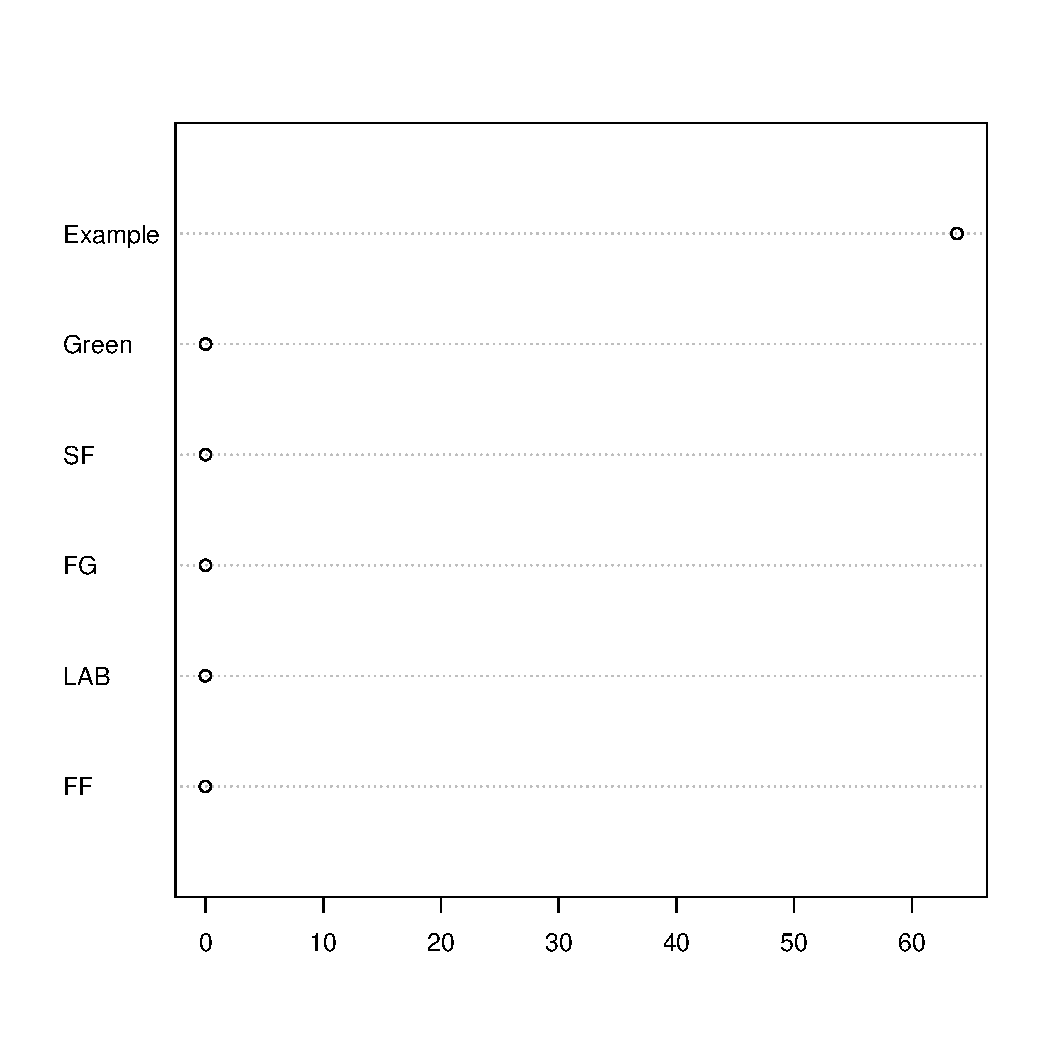
\includegraphics[width=\maxwidth]{figures/minimal-unnamed-chunk-14} 

}



\end{knitrout}

We will discuss analysis techniques in more detail later. The dfm command has many optional arguments for applying standard pre-processing techniques to texts. We can choose to apply word stemming, which will sum together counts of words that have a common morphological root --- for example \textit{earn, earning, earns} and \textit{earned} will all be counted together under the single stem \textit{earn*}. Again, this is easy to see by making a new matrix and inspecing it with \texttt{View()}

\begin{knitrout}\footnotesize
\definecolor{shadecolor}{rgb}{0.969, 0.969, 0.969}\color{fgcolor}\begin{kframe}
\begin{alltt}
\hlstd{docMatStems} \hlkwb{<-} \hlkwd{dfm}\hlstd{(ieBudgets2010,} \hlkwc{stem}\hlstd{=}\hlnum{TRUE}\hlstd{)}
\end{alltt}
\begin{verbatim}
## Creating dfm: ...
\end{verbatim}


{\ttfamily\noindent\itshape\color{messagecolor}{\#\# Loading required package: SnowballC}}\begin{verbatim}
##  stemming ... done.
\end{verbatim}
\begin{alltt}
\hlstd{docMatStems[}\hlnum{1}\hlopt{:}\hlnum{5}\hlstd{,}\hlnum{1}\hlopt{:}\hlnum{5}\hlstd{]}
\end{alltt}
\begin{verbatim}
##                                       words
## docs                                   V1  €  —   a abandon
##   2010_BUDGET_01_Brian_Lenihan_FF.txt   3 75  4 180       0
##   2010_BUDGET_02_Richard_Bruton_FG.txt  0 18  5  96       1
##   2010_BUDGET_03_Joan_Burton_LAB.txt    1 48 11 165       1
##   2010_BUDGET_04_Arthur_Morgan_SF.txt   2 42  7 144       1
##   2010_BUDGET_05_Brian_Cowen_FF.txt     3 38  7 161       0
\end{verbatim}
\end{kframe}
\end{knitrout}

\subsubsection{Importing to and exporting from \textsf{tm}}

The \textsf{tm} package uses a sparse matrix format to store document-frequency matrices. Word frequency follows a power-law distribution (Zipf's law) --- a few words are very frequent, while most words in the total corpus vocabulary don't occur at all in the a particular document, particularly if the length of each document is a small fraction of the length of the total corpus.  The result is that most cells in a document-frequency matrix have a value of zero. 

In order to use less storage space, \textsf{tm} only stores the row and column numbers where the value is not zero. This is known as a simple triplet representation. To make use of functions from \textsf{tm}, we must first convert the quanteda dfm into this format. 

\begin{knitrout}\footnotesize
\definecolor{shadecolor}{rgb}{0.969, 0.969, 0.969}\color{fgcolor}\begin{kframe}
\begin{alltt}
\hlstd{tmMat}\hlkwb{<-} \hlkwd{dfm2tmformat}\hlstd{(partMat)}
\end{alltt}


{\ttfamily\noindent\itshape\color{messagecolor}{\#\# Loading required package: slam\\\#\# Loading required package: tm\\\#\# Loading required package: NLP}}\begin{alltt}
\hlkwd{names}\hlstd{(tmMat)}
\end{alltt}
\begin{verbatim}
## [1] "i"        "j"        "v"        "nrow"     "ncol"     "dimnames"
\end{verbatim}
\end{kframe}
\end{knitrout}

% \singlespacing
\bibliographystyle{apsr}
\bibliography{QUANTESS}

\end{document}

In order to perform statistical analysis such as document scaling, we must extract a matrix containing the frequency of each word type from in document. In quanteda, we use the dfm function to produce such a matrix. \footnote{dfm stands for document-feature matrix --- we say ``feature'' instead of word, as it is sometimes useful to represent documents by features other than their word frequency.}

\begin{knitrout}\footnotesize
\definecolor{shadecolor}{rgb}{0.969, 0.969, 0.969}\color{fgcolor}\begin{kframe}
\begin{alltt}
\hlstd{docMat} \hlkwb{<-} \hlkwd{dfm}\hlstd{(ieBudgets2010)}
\end{alltt}
\begin{verbatim}
## Creating dfm: ... done.
\end{verbatim}
\begin{alltt}
\hlstd{docMat[}\hlnum{1}\hlopt{:}\hlnum{5}\hlstd{,}\hlnum{1}\hlopt{:}\hlnum{5}\hlstd{]}
\end{alltt}
\begin{verbatim}
##                                       words
## docs                                    €  —   a abandoned abandoning
##   2010_BUDGET_01_Brian_Lenihan_FF.txt  75  4 143         0          0
##   2010_BUDGET_02_Richard_Bruton_FG.txt 18  5  82         1          0
##   2010_BUDGET_03_Joan_Burton_LAB.txt   48 11 129         1          0
##   2010_BUDGET_04_Arthur_Morgan_SF.txt  42  7 115         0          1
##   2010_BUDGET_05_Brian_Cowen_FF.txt    38  7 122         0          0
\end{verbatim}
\end{kframe}
\end{knitrout}

We can now score and plot the documents using a statistical scaling technique, for example correspondence analysis.

\begin{knitrout}\footnotesize
\definecolor{shadecolor}{rgb}{0.969, 0.969, 0.969}\color{fgcolor}\begin{kframe}
\begin{alltt}
\hlkwd{library}\hlstd{(ca)}
\hlstd{model} \hlkwb{<-} \hlkwd{ca}\hlstd{(}\hlkwd{t}\hlstd{(docMat),}\hlkwc{nd}\hlstd{=}\hlnum{1}\hlstd{)}
\hlkwd{dotchart}\hlstd{(model}\hlopt{$}\hlstd{colcoord[}\hlkwd{order}\hlstd{(model}\hlopt{$}\hlstd{colcoord[,}\hlnum{1}\hlstd{]),}\hlnum{1}\hlstd{],} \hlkwc{labels} \hlstd{= model}\hlopt{$}\hlstd{colnames[}\hlkwd{order}\hlstd{(model}\hlopt{$}\hlstd{colcoord[,}\hlnum{1}\hlstd{])])}
\end{alltt}
\end{kframe}

{\centering 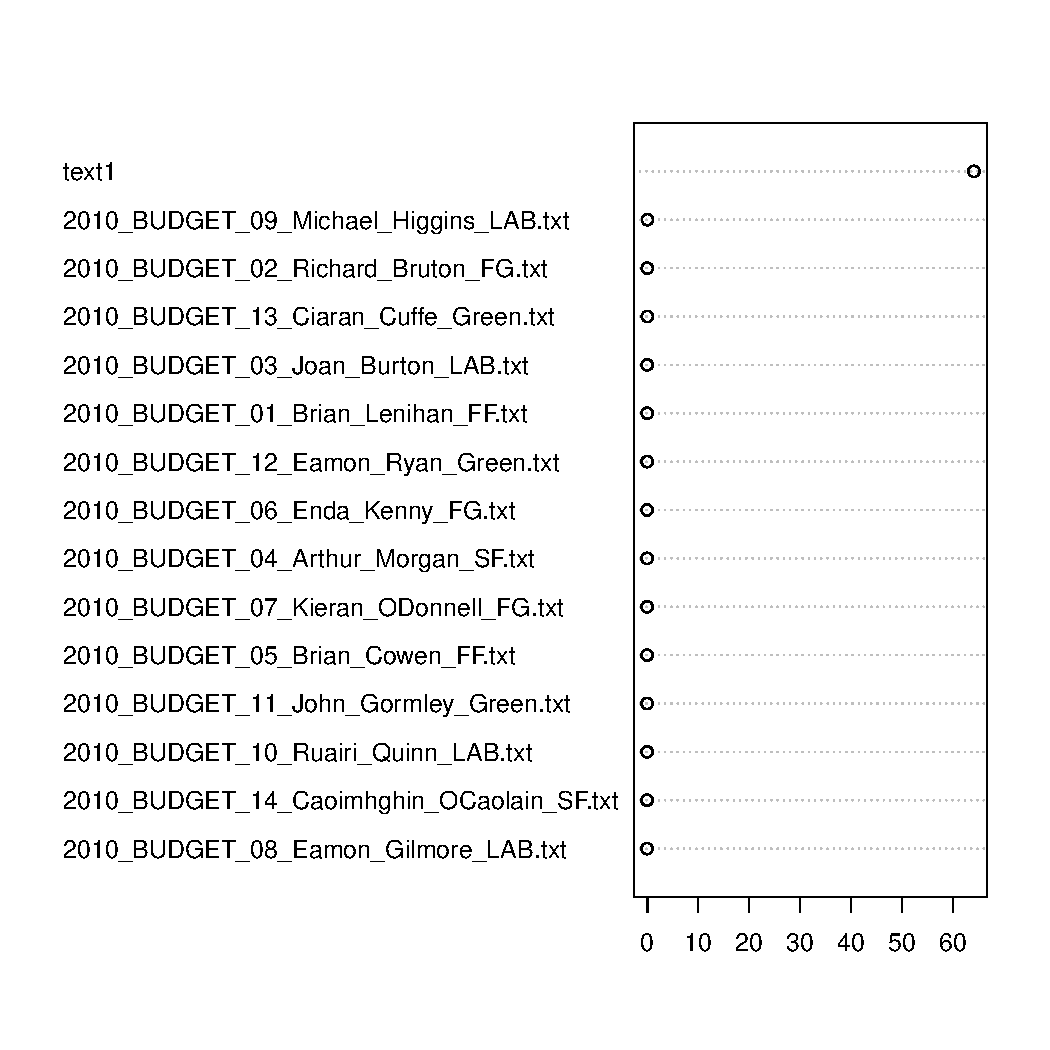
\includegraphics[width=\maxwidth]{figures/minimal-unnamed-chunk-18} 

}



\end{knitrout}

This plot indicates the position
of each of the documents. We can group documents by their attribute values when creating the word-frequency matrix: 

\begin{knitrout}\footnotesize
\definecolor{shadecolor}{rgb}{0.969, 0.969, 0.969}\color{fgcolor}\begin{kframe}
\begin{alltt}
\hlstd{partyMat} \hlkwb{<-} \hlkwd{dfm}\hlstd{(ieBudgets2010,} \hlkwc{group}\hlstd{=}\hlstr{"party"}\hlstd{)}
\end{alltt}
\begin{verbatim}
## Creating dfm: ... aggregating by group: party...complete ... done.
\end{verbatim}
\begin{alltt}
\hlstd{partyMat[,}\hlnum{1}\hlopt{:}\hlnum{5}\hlstd{]}
\end{alltt}
\begin{verbatim}
##        words
## docs      €  —   a abandoned abandoning
##   FF     35  5  78         0          0
##   FG     31  9 162         0          0
##   Green 108 23 326         2          1
##   LAB    75  9 288         0          0
##   SF     85  4 159         0          0
\end{verbatim}
\end{kframe}
\end{knitrout}

which allows us to scale according to a particular party or year, for example:

\begin{knitrout}\footnotesize
\definecolor{shadecolor}{rgb}{0.969, 0.969, 0.969}\color{fgcolor}\begin{kframe}
\begin{alltt}
\hlstd{partyModel} \hlkwb{<-} \hlkwd{ca}\hlstd{(}\hlkwd{t}\hlstd{(partyMat),}\hlkwc{nd}\hlstd{=}\hlnum{1}\hlstd{)}
\hlkwd{dotchart}\hlstd{(partyModel}\hlopt{$}\hlstd{colcoord[}\hlkwd{order}\hlstd{(partyModel}\hlopt{$}\hlstd{colcoord[,}\hlnum{1}\hlstd{]),}\hlnum{1}\hlstd{],} \hlkwc{labels} \hlstd{= partyModel}\hlopt{$}\hlstd{colnames[}\hlkwd{order}\hlstd{(partyModel}\hlopt{$}\hlstd{colcoord[,}\hlnum{1}\hlstd{])])}
\end{alltt}
\end{kframe}

{\centering 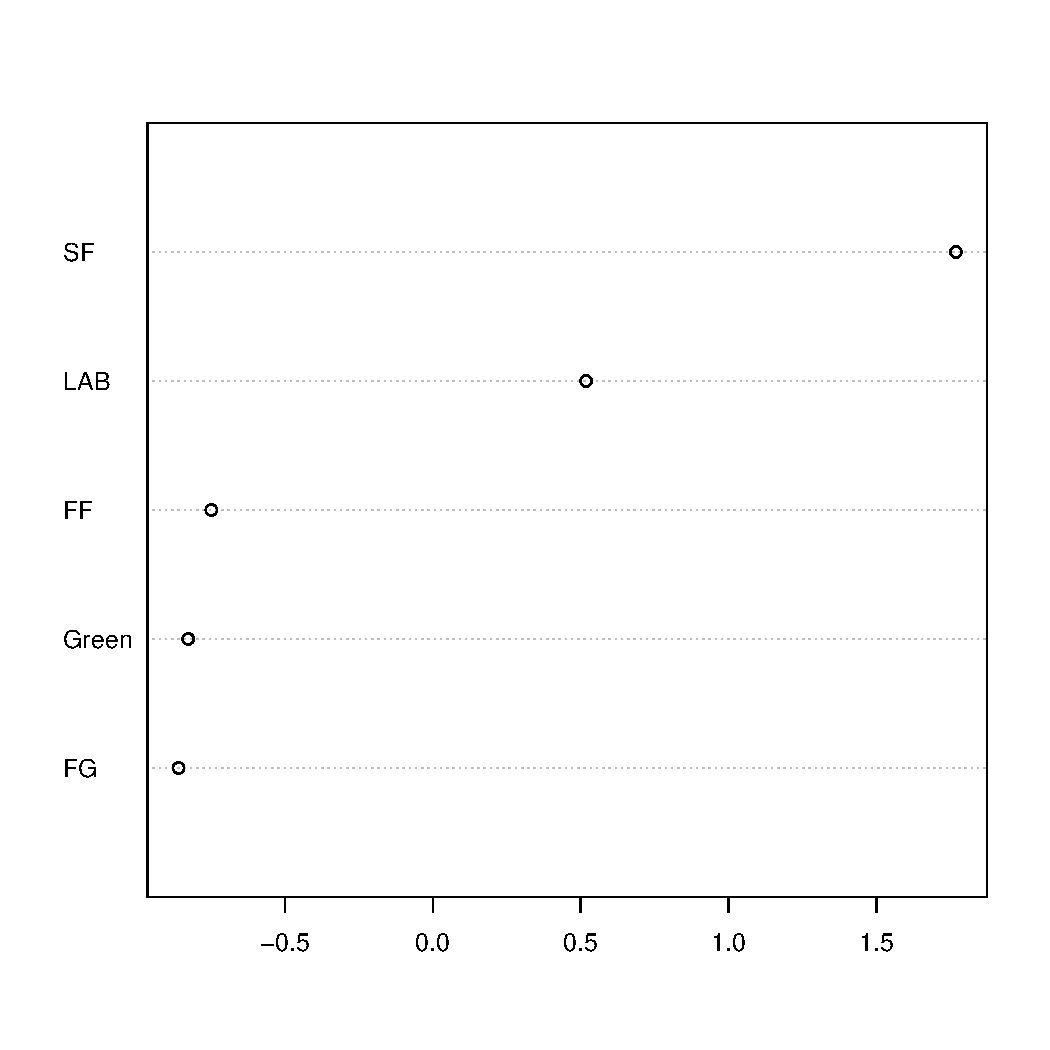
\includegraphics[width=\maxwidth]{figures/minimal-unnamed-chunk-20} 

}



\end{knitrout}



